%----------------------------------------------------------------------
% 設計方法
%----------------------------------------------------------------------

\chapter{Proposed Method}\label{chap:method}

The proposed method introduces consistency objectives into the MTP training process while keeping the model architecture identical to the original MTP design. The overall training objective consists of the original MTP cross-entropy loss, Selective Distribution Consistency (SDC), and Latent Consistency Matching (LCM).

\section{MTP Training Objective}\label{sec:3-mtp_training_objective}

Given $K$ prediction heads, each head predicts a token at a different future position and is optimized using the cross-entropy loss with its corresponding ground-truth token. The baseline MTP objective is defined as

\begin{equation}
    \mathcal{L}_{\mathrm{MTP}}=\sum_{k=1}^{K}\mathcal{L}_{\mathrm{CE}}^{(k)},
\end{equation}

where $\mathcal{L}_{\mathrm{CE}}^{(k)}$ denotes the cross-entropy loss of the $k$-th prediction head for its corresponding future target token. This objective is retained as the primary token prediction loss in the proposed training framework.

\section{Selective Distribution Consistency}\label{sec:3-selective_distribution_consistency}

\begin{figure}[hpbt]
    \centering
    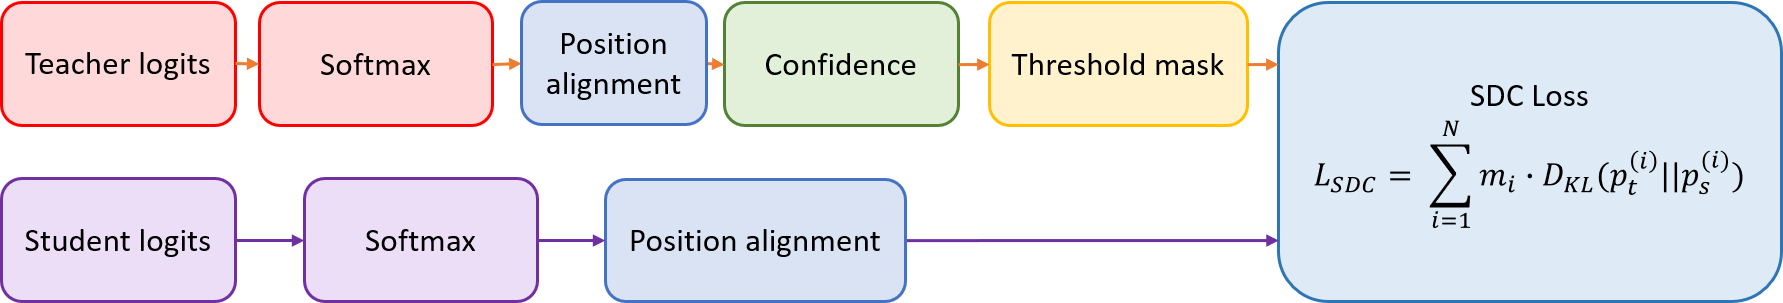
\includegraphics[width=\textwidth]{Figures/sdc_block_diagram.png}
    \caption{SDC block diagram.}
    \label{fig:sdc_block_diagram}
\end{figure}

Selective Distribution Consistency (SDC) aligns the output probability distributions of the student heads (Heads 2--$K$) with the teacher head (Head 1). Since different prediction heads correspond to different future offsets, the teacher and student predictions are first position-aligned such that they correspond to the same target token. Specifically, the prediction of Head $k$ at position $i$ is aligned with the prediction of Head 1 at position $i+k-1$.

For each token position, the teacher logits are first converted into a probability distribution using softmax:

\begin{equation}
    P_{t}^{(i)}=\operatorname{softmax}\left(z_{t}^{(i)}\right),
\end{equation}

where $P_{t}^{(i)}$ denotes the probability distribution produced by the teacher head (Head 1) at position $i$.

The confidence of the teacher prediction is then estimated using its normalized entropy:

\begin{equation}
    c_{i}=1-\frac{H\left(P_{t}^{(i)}\right)}{\log(V)},
\end{equation}

where $H(\cdot)$ denotes the entropy of the teacher probability distribution and $V$ is the vocabulary size. A higher $c_{i}$ indicates a more confident teacher prediction.

A confidence threshold $\tau$ is subsequently applied to construct a binary mask:

\begin{equation}
    m_{i}=\begin{cases}
                    1, & \text{if } c_{i} > \tau, \\
                    0, & \text{otherwise}.
                \end{cases}
\end{equation}

Thus, only token positions whose teacher confidence exceeds $\tau$ participate in consistency learning, while low-confidence positions are excluded from the SDC objective.

For the selected positions, the student probability distribution is encouraged to match the corresponding position-aligned teacher distribution by minimizing the KL divergence:

\begin{equation}
    \mathcal{L}_{\mathrm{SDC}}^{(k)}=\frac{1}{N_k}\sum_{i}m_{i+k-1}D_{\mathrm{KL}}\left(P_{t}^{(i+k-1)} \parallel P_{s}^{(i,k)}\right),
\end{equation}

where $P_{t}^{(i+k-1)}$ and $P_{s}^{(i,k)}$ denote the position-aligned teacher and student probability distributions corresponding to the same target token, respectively, and $N_k$ denotes the number of positions selected by the confidence mask for the $k$-th student head.

The overall SDC objective is defined as

\begin{equation}
    \mathcal{L}_{\mathrm{SDC}}=\sum_{k=2}^{K}\mathcal{L}_{\mathrm{SDC}}^{(k)}.
\end{equation}

This selective mechanism restricts distribution consistency learning to positions with sufficiently reliable teacher predictions.

\begin{algorithm}[htbp]
\caption{Selective Distribution Consistency}
\label{alg:sdc}

\KwIn{
Teacher logits $\{z_t^{(i)}\}$ from Head 1,
student logits $\{z_s^{(i,k)}\}_{k=2}^{K}$,
confidence threshold $\tau$
}

\KwOut{SDC loss $\mathcal{L}_{\mathrm{SDC}}$}

$\mathcal{L}_{\mathrm{SDC}} \leftarrow 0$\;

\ForEach{teacher position $i$}{
    $P_t^{(i)} \leftarrow \operatorname{softmax}\left(z_t^{(i)}\right)$\;
    
    $c_i \leftarrow
    1-\dfrac{H\left(P_t^{(i)}\right)}{\log V}$\;
    
    $m_i \leftarrow \mathbb{I}(c_i > \tau)$\;
}

\For{$k \leftarrow 2$ \KwTo $K$}{
    Align Head $k$ at position $i$ with Head 1 at position $i+k-1$\;
    
    $\mathcal{I}_k
    \leftarrow
    \{i \mid m_{i+k-1}=1\}$\;
    
    $N_k \leftarrow |\mathcal{I}_k|$\;
    
    $\mathcal{L}_{\mathrm{SDC}}^{(k)}
    \leftarrow
    \dfrac{1}{N_k}
    \displaystyle\sum_{i\in\mathcal{I}_k}
    D_{\mathrm{KL}}
    \left(
    P_t^{(i+k-1)}
    \parallel
    P_s^{(i,k)}
    \right)$\;
    
    $\mathcal{L}_{\mathrm{SDC}}
    \leftarrow
    \mathcal{L}_{\mathrm{SDC}}
    +
    \mathcal{L}_{\mathrm{SDC}}^{(k)}$\;
}

\Return{$\mathcal{L}_{\mathrm{SDC}}$}\;

\end{algorithm}

\section{Latent Consistency Matching}\label{sec:3-latent_consistency_matching}
Latent Consistency Matching (LCM) applies consistency learning at the latent representation level. The same position-alignment strategy used in SDC is applied to the hidden representations before latent consistency matching. Specifically, the hidden representation produced by the $k$-th student head is aligned with the representation produced by Head 1 that corresponds to the same target token.

For the $k$-th student head, the LCM loss is defined as

\begin{equation}
    \mathcal{L}_{\mathrm{LCM}}^{(k)}=\frac{1}{S_k D}\sum_{i=1}^{S_k}\sum_{d=1}^{D}\left(h_{t,i,d}^{(k)}-h_{s,i,d}^{(k)}\right)^2,
\end{equation}

where $h_{t,i,d}^{(k)}$ and $h_{s,i,d}^{(k)}$ denote the position-aligned teacher and student hidden representations, respectively, $S_k$ denotes the number of valid aligned token positions for the $k$-th student head, and $D$ denotes the hidden dimension.

The overall LCM objective is defined as

\begin{equation}
    \mathcal{L}_{\mathrm{LCM}}=\sum_{k=2}^{K}\mathcal{L}_{\mathrm{LCM}}^{(k)}.
\end{equation}

While SDC constrains the prediction heads at the output distribution level, LCM provides an additional consistency constraint on their position-aligned latent representations.
\section{Joint Training Objective}\label{sec:3-joint_training_objective}

The final training objective combines the original MTP loss with the two consistency objectives:

\begin{equation}\label{equ:joint_training_objective}
    \mathcal{L}_{\mathrm{total}} = \mathcal{L}_{\mathrm{MTP}} + \lambda_{\mathrm{SDC}}\mathcal{L}_{\mathrm{SDC}} + \lambda_{\mathrm{LCM}}\mathcal{L}_{\mathrm{LCM}},
\end{equation}

where $\lambda_{\mathrm{SDC}}$ and $\lambda_{\mathrm{LCM}}$ control the contributions of SDC and LCM, respectively.

During training, the teacher outputs are detached when computing the consistency objectives. Therefore, SDC and LCM use Head 1 as the reference to optimize Heads 2--$K$, while the original cross-entropy objective continues to optimize all prediction heads.
